\documentclass{article}
\usepackage[utf8]{inputenc}
\usepackage[margin=1.1in]{geometry}
\usepackage{graphicx}
\usepackage{tikz}
\usepackage{caption}
\usepackage{textgreek}
\usepackage{minted}
\usepackage{enumitem}
\usepackage{hyperref}
\usepackage{ulem}
\begin{document}
\author{\href{https://github.com/beasrodrigues24}{Beatriz Rodrigues} \orcidID{\textit{(a93230)}} \and \href{https://github.com/franl08}{Francisco Neves} \orcidID{\textit{(a93202)}} \and \href{https://github.com/zer0-5}{Guilherme Fernandes}\orcidID{\textit{(a93216)}}}
\date{27 de Março 2022}
\title{\LARGE \textbf{yaPP}\\
    \Large Processamento de Linguagens\\
    \large Grupo 24 \\
}
\maketitle
\section{Introdução}
O presente relatório é relativo à realização do primeiro trabalho prático da UC de Processamento de Linguagens na Universidade do Minho e consequente implementação de uma aplicação designada por yaPP (Yet Another PreProcessor).\\
 O desenvolvimento deste trabalho prático teve como principais objetivos os seguintes pontos: 
\begin{itemize}
\item Aumentar a experiência de uso do ambiente Linux e de algumas ferramentas de apoio à programação;
\item Aumentar a capacidade de escrever Expressões Regulares (ER) para descrição de padrões em \textit{streams} de texto;
\item Desenvolver, a partir de Expressões Regulares, sistemática e automaticamente, Processadores de Linguagens Regulares, que encontrem ou transformem textos com base no conceito de regras de produção Condição-Ação;
\item Utilizar o \textit{Python} e os seus módulos \textit{re} e \textit{ply} para gerar os filtros de texto;
\end{itemize}
 Tendo isto em conta, o grupo decidiu optar pela escolha do segundo tema proposto para a realização do trabalho prático, ou seja, pelo desenvolvimento de um pré-processador para \textit{LaTeX} ou \textit{HTML}, pois, foi considerado que este seria o tema que traria mais benefício de ser explorado e uma possível grande utilidade no nosso quotidiano.\\
 É, no entanto, imperativa a perceção de aquilo que é um pré-processador, para uma consequente boa aplicação dos seus conceitos. Desta forma, podemos afirmar que um pré-processador permite que através de notações mais leves e simples (de preferência independentes do tipo de documento final) para que, posteriormente, se recorra ao pré-processamento para substituir a notação ligeira, abreviada, pelas marcas finais corretas. Como exemplos de pré-processadores podemos considerar o \textit{PPP}, desenvolvido por José Carlos Ramalho, ou a mais atual e bem conhecida linguagem \textit{MarkDown} para a construção de páginas \textit{HTML}.\\
 Para o desenvolvimento do yaPP, foi utilizada linguagem de programação \textit{Python} e recorreu-se aos seus módulos \textit{re} e \textit{ply} de forma a gerar os filtros de texto adequados a partir das Expressões Regulares que encontrassem.\\
 Visto que um dos objetivos de um pré-processador é permitir que um mesmo ficheiro possa ser pré-processado para diversas linguagens, foi ainda decidido, que seria dada prioridade ao desenvolvimento de um pré-processador focado em \textit{HTML}, no entanto, deveria ainda ser capaz de efetuar o pré-processamento para \textit{LaTeX} se assim o utilizador pretendesse.\section{Descrição do Problema}
Para o desenvolvimento do pré-processador, foi proposto que fosse desenvolvida uma linguagem própria com uma notação específica de forma a abreviar e suportar os seguintes pontos: 
\begin{enumerate}
\item Formatação: \textbf{negrito}, \textit{itálico}, \underline{sublinhado};
\item Vários níveis de títulos;
\item Listas de tópicos (items) não-numerados, numerados ou tipos de entrada de um dicionário;
\item Inclusão de imagens;
\item Inclusão e formatação de tabelas;
\end{enumerate}
\\
 No entanto, foi ainda encorajada a implementação de outros pontos que fossem considerados necessários ou criativos.\\
 Após isso, seria ainda necessário, recorrendo ao módulo \textit{ply} do \textit{Python} que fosse criado um processador de forma a transformar a notação decidida em notação de \textit{LaTeX} ou \textit{HTML}.\\
 Devia, ainda, ser previsto o aninhamento e a combinação dos diversos componentes anteriormente enumerados.\section{Solução Desenvolvida}
Tendo em conta os diversos requisitos e as diversas utilidades que um pré-processador deve apresentar, foram implementadas todas as funcionalidades obrigatórias e ainda outras consideradas úteis por parte do grupo de desenvolvimento. Assim, temos que foram implementadas as seguintes funcionalidades: \subsection{Funcionalidades \textit{inline}}
Consideramos funcionalidades \textit{inline} aquelas que se tratam de funcionalidades de uma linha, ao invés de grandes blocos.\\
 A este nível foram implementadas as seguintes funcionalidades: 
\begin{itemize}
\item \textbf{Título} - é possível indicar o título do documento utilizando [\textit{t} título];
\item \textbf{Negritos} - é possível tornar texto negrito utilizando [\textit{b} texto];
\item \textbf{Itálicos} - é possível tornar texto itálico utilizando [\textit{i} texto];
\item \textbf{Sublinhados} - é possível tornar texto sublinhado utilizando [\textit{u} texto];
\item \textbf{Imagens} - é possível colocar imagess utilizando [\textit{img} srclink [\textit{name} nome] [\textit{w} largura] [\textit{h} altura]] (para LaTeX, os campos w e h não são aplicáveis);
\end{itemize}
 Além destas, consideradas obrigatórias, foram ainda implementadas as seguintes por serem consideradas úteis por parte do grupo de desenvolvimento: 
\begin{itemize}
\item \textbf{Riscado} - texto riscado utilizando [\textit{stk} texto];
\item \textbf{Subscrito} - texto subscrito utilizando [\textit{sub} texto];
\item \textbf{Sobrescrito} - texto sobrescrito utilizando [\textit{sup} texto];
\item \textbf{Código \textit{Inline}} - código \textit{inline} utilizando [\textit{c} código];
\item \textbf{\textit{Hyperlinks}} - \textit{hyperlinks} utilizando [\textit{href} link [\textit{name} nome]];
\item \textbf{Caracteres Especiais} - caracteres especiais (como letras gregas) utilizando [\textit{sp} nome do caractere] (para LaTeX, apenas letras gregas);
\item \textbf{Comentários} - comentários utilizando \textit{//};
\item \textbf{\textit{Newlines}} - newlines utilizando duas vezes \textbackslashn;
\item \textbf{Caracteres \textit{Escaped}} - para utilizar [ ou ], é necessário inserir \textbackslash antes do caractere desejado;
\end{itemize}
 \subsection{Funcionalidades em blocos}
A este nível, foram implementadas as seguintes funcionalidades:
\begin{description}
\item[\textbf{Secções}]\\
Secções e vários níveis de títulos com:\\
\textit{[sec} título\\
\textit{texto da secção}\\
para terminar o bloco utiliza-se:\\
\textit{sec]}
\item[\textbf{Listas não-numeradas}]\\
Listas não-numeradas utilizando:\\
\textit{[list}\\
\textit{[item} conteúdo do item\textit{]}\\
para terminar a lista utiliza-se:\\
\textit{list]}
\item[\textbf{Listas ordenadas}]\\
Listas ordenadas por caracteres ou números utilizando:\\
\textit{[ordlist} (1 ou a ou A)\\
\textit{[item} conteúdo do item\textit{]}\\
para terminar a lista utiliza-se:\\
\textit{ordlist]}
\item[\textbf{Listas dicionário}]\\
Listas dicionário utilizando:\\
\textit{[dsclist}\\
\textit{[obj} nome do item\textit{]}\\
\textit{[dsc} primeira descrição\textit{]}\\
\textit{[dsc} segunda descrição\textit{]}\\
para terminar a lista utiliza-se:\\
\textit{dsclist\textit{]}}
\item[\textbf{Tabelas}]\\
Tabelas utilizando:\\
\textit{[table} número de colunas\\
\textit{[row} [\textit{h} A][\textit{h} B]]\\
\textit{[row} [\textit{e} a][\textit{e} b]]\\
para terminar a tabela utiliza-se:\\
\textit{table}]
\end{description}
 Além destas, consideradas obrigatórias, foram ainda implementadas as seguintes por serem consideradas úteis por parte do grupo de desenvolvimento:
\begin{description}
\item[\textbf{Blocos de Código}]\\
Blocos de código utilizando:\\
\textit{[code} code linguagem\\
\textit{código}\\
para terminar o bloco utiliza-se:\\
\textit{code]}
\item[\textbf{\textit{Raw Block}}]\\
Blocos de código \textit{raw} (permite escrever \textit{LaTeX} ou \textit{HTML} diretamente) utilizando:\\
\textit{[raw}\\
\textit{código}\\
para terminar o bloco utiliza-se:\\
\textit{raw]}
\item[\textbf{Tabelas com bordas}]\\
Tabelas com bordas utilizando:\\
\textit{[btable} número de colunas\\
\textit{[row} [\textit{h} A][\textit{h} B]]\\
\textit{[row} [\textit{e} a][\textit{e} b]]\\
para terminar a tabela utiliza-se:\\
\textit{table}]\\
Esta tabela só se diferencia da sem bordas em \textit{HTML}.
\end{description}
 Além destas, consideramos ainda importante destacar que a aplicação é capaz de efetuar o pré-processamento tanto para \textit{HTML} como para \textit{LaTeX} de forma a permitir que um único documento seja capaz de gerar um documento \textit{LaTeX} e outro \textit{HTML}.\\
 \subsection{Implementação}
\subsubsection{\textit{Tokens} e \textit{Start Conditions}}
Para ser possível a gestão das várias funcionalidades implementadas, foram criados vários \textit{tokens}: 
\begin{itemize}
\item \texttt{BOLD};
\item \texttt{ITALIC};
\item \texttt{UNDERLINE};
\item \texttt{CINLINE};
\item \texttt{SUBSCRIPT};
\item \texttt{SUPERSCRIPT};
\item \texttt{STRIKEOUT};
\item \texttt{HREF};
\item \texttt{CODE};
\item Entre outros...
\end{itemize}
\\
 Para além disso, pela mesma razão, foram também colocadas várias \textit{start conditions} que podem ser \textit{inclusive} ou \textit{exclusive}. Diferenciam-se pelo facto de que as exclusivas não prevêem aninhamento entre estados. Alguns exemplos são: 
\begin{itemize}
\item \texttt{('section', 'inclusive')};
\item \texttt{('list', 'exclusive')};
\item \texttt{('item', 'inclusive')};
\item \texttt{('superscript', 'inclusive')};
\item \texttt{('strikeout', 'inclusive')};
\item Entre outros...
\end{itemize}
\\
 Estas \textit{conditions} funcionam sob a forma de uma \textit{stack}, a partir da qual é possível gerir o facto de podermos ter estados dentro de outros estados e, por isso, permitir, por exemplo, negritos dentro de itálicos e conter subsecções dentro de secções. \subsubsection{Expressões Regulares}
Através de expressões regulares, podemos associar a sintaxe prevista aos \textit{tokens} que achamos necessários. Desta forma, é possível, junto com as \textit{start conditions}, detetar qual será o \textit{output} correspondente ao \textit{input} do utilizador.\\
 Um exemplo é a gestão das secções. Esta utiliza uma variável auxiliar que permite sabermos se a secção corresponde na verdade a uma subsecção. Para além disso, o título da secção é capturado como texto normal, uma vez que a \textit{start condition} é inclusiva.\\
 \begin{minted}{python}
def t_SECTION(t):
    r'\[sec\ '
    t.lexer.header_num += 1
    t.value = "\n\\"
    for x in range(1, t.lexer.header_num):
        t.value += "sub"
    t.value += "section{"
    t.lexer.push_state('section')
    t.lexer.push_state('sectiontitle')
    return t
def t_sectiontitle_END(t):
    r'\n\s*'
    t.value = "}\n"
    t.lexer.pop_state()
    return t
def t_section_END(t):
    r'\s*sec\]\n?'
    t.lexer.pop_state()
    t.lexer.header_num -= 1
\end{minted}
 \subsection{Controlador}
De forma a conseguirmos gerir a conversão para \textit{HTML} ou \textit{LaTeX} de acordo com a vontade do utilizador, foi necessário implementar um controlador que redirecionasse para as funções correspondentes. Para isso, foi implementado um ficheiro \textit{yapp.py}, a partir do qual se faz o redirecionamento para o tipo de conversão desejada, a partir de uma flag que deve ser inserida pelo utilizador (\texttt{-t latex} ou \texttt{-t html}). Caso não seja indicada, o \textit{default} é \textit{HTML}. O utilizador deve indicar ainda o nome do ficheiro de \textit{input} e o nome do ficheiro de \textit{output}. Segue-se um exemplo de execução do programa: \texttt{python yapp.py manual.ya manual.html -t html}. Após receber a informação acerca do tipo de conversão, o programa inicializa o pré-processador e o \textit{lexer} e as suas variáveis, para, de seguida, corresponder cada \textit{token} à ação correspondente. Uma das variáveis corresponde ao \textit{Converter}, que poderá ser \textit{HTML converter} ou \textit{LaTeX converter}, permitindo que, por exemplo, quando é detetado o início de uma porção de texto a negrito, seja obtido a marca textual que inicia o negrito na linguagem final.\newpage
\section{Testes Efetuados}
De forma a comprovarmos a viabilidade e utilidade da aplicação desenvolvida, foram escritos diversos documentos de forma a verificar os diversos aspetos da nossa aplicação.\\
 \subsection{Manual da Aplicação}
De forma a facilitar a utilização deste pré-processador, foi escrito um manual de utilização na linguagem desenvolvida. Por conveniência, serviu ainda como um teste ao fazermos a conversão para HTML e latex.\\
 
\begin{figure}[!ht]
\centering
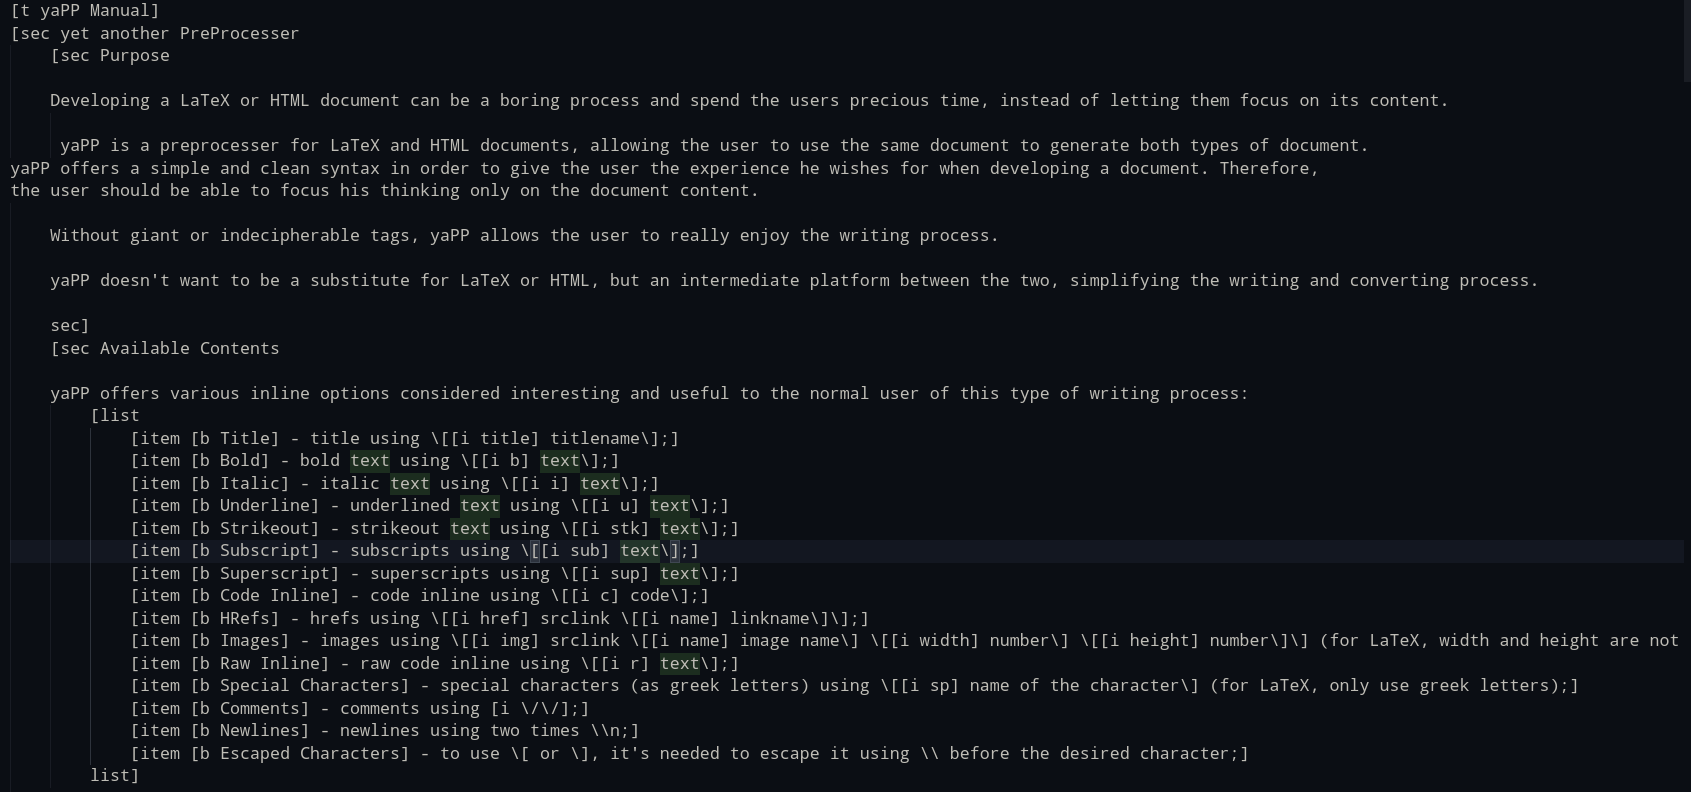
\includegraphics[width=\textwidth]{images/manualYA.png}
\caption{Manual em .YA}
\end{figure}
\\
 
\begin{figure}[!ht]
\centering
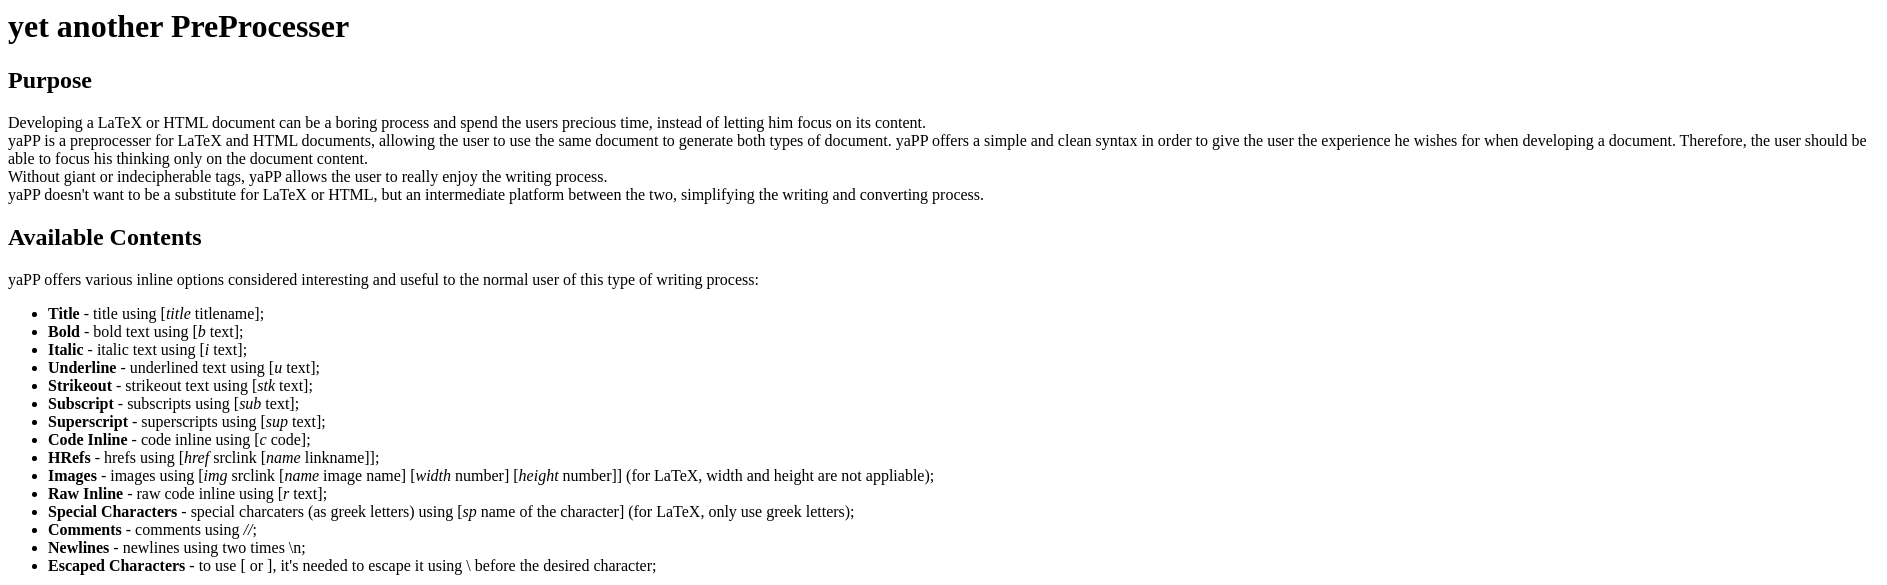
\includegraphics[width=\textwidth]{images/manualHTML.png}
\caption{Manual em HTML}
\end{figure}
\\
 
\begin{figure}[!ht]
\centering
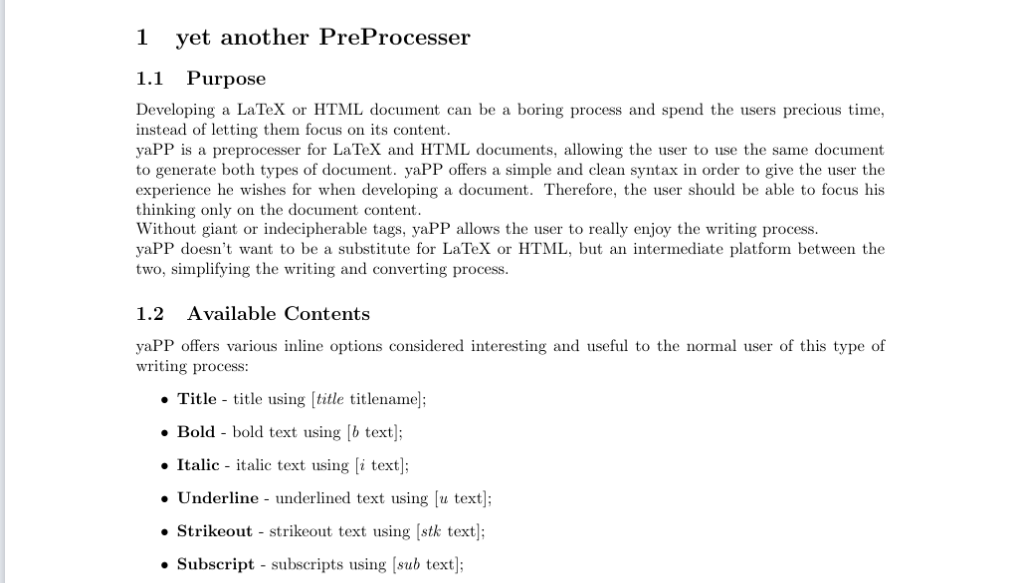
\includegraphics[width=\textwidth]{images/manualTEX.png}
\caption{Manual em Latex}
\end{figure}
 \clearpage
 \subsection{Apontamentos}
Para além disso, verificamos que também é possível escrever apontamentos de forma legível e elegante, com recurso à funcionalidade extra que adicionamos, os \textit{code blocks}.\\
 
\begin{figure}[!ht]
\centering
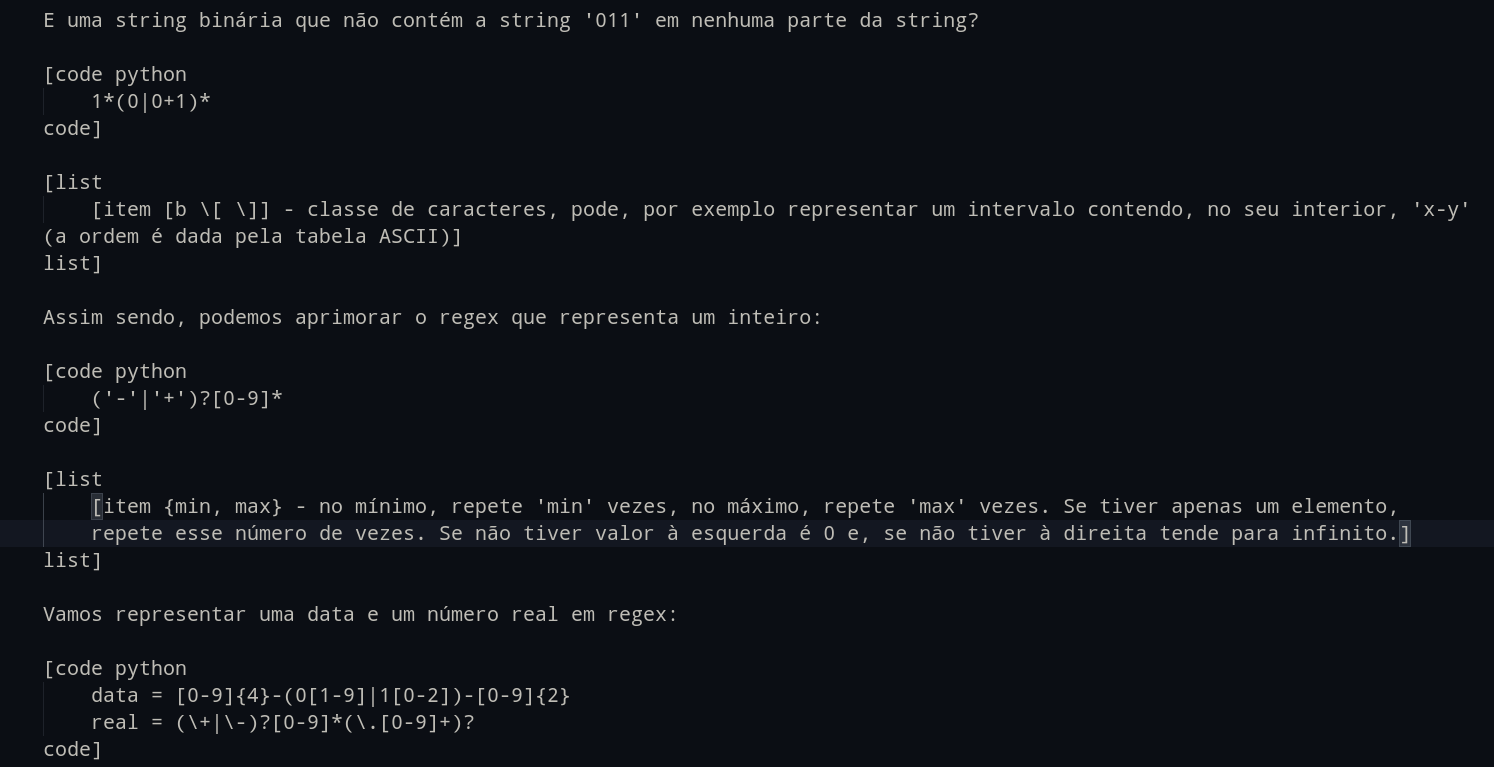
\includegraphics[width=\textwidth]{images/apontamentosYA.png}
\caption{Apontamentos em .YA}
\end{figure}
\\
 
\begin{figure}[!ht]
\centering
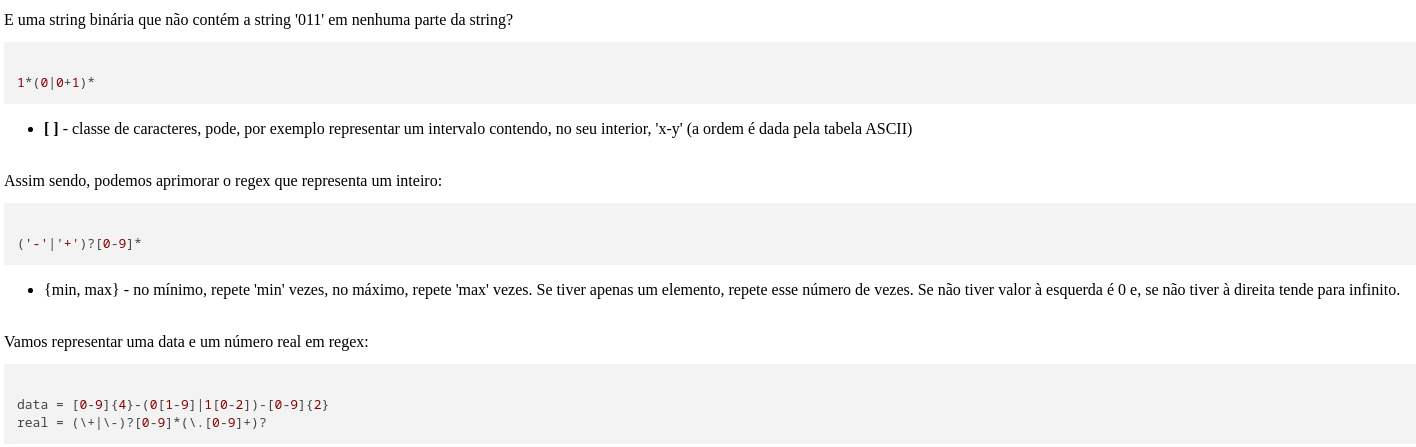
\includegraphics[width=\textwidth]{images/apontamentosHTML.png}
\caption{Apontamentos em HTML}
\end{figure}
\\
 
\begin{figure}[!ht]
\centering
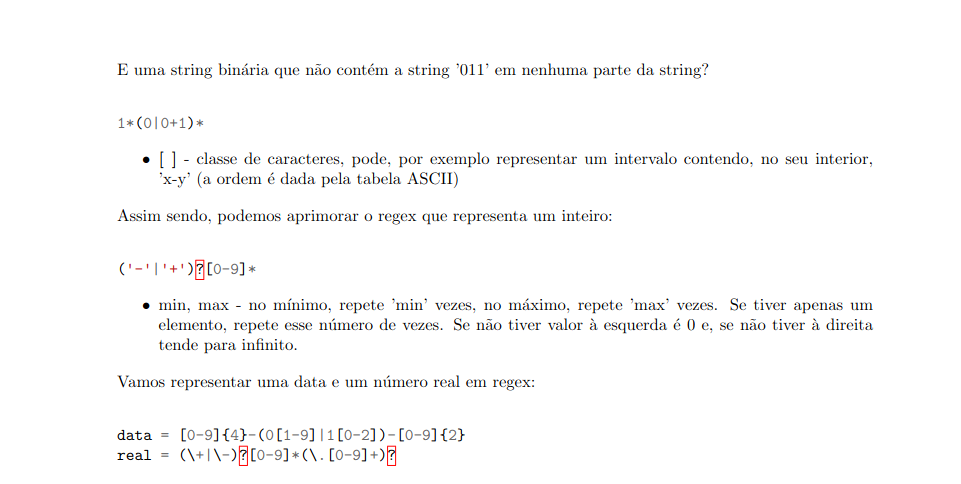
\includegraphics[width=\textwidth]{images/apontamentosTEX.png}
\caption{Apontamentos em Latex}
\end{figure}
 \clearpage
 \subsection{Relatório de Desenvolvimento do presente Trabalho}
Como o teste mais relevante, foi decidido escrever o relatório de desenvolvimento do projeto na linguagem desenvolvida, de forma a detetar possíveis falhas.\\
 
\begin{figure}[!ht]
\centering
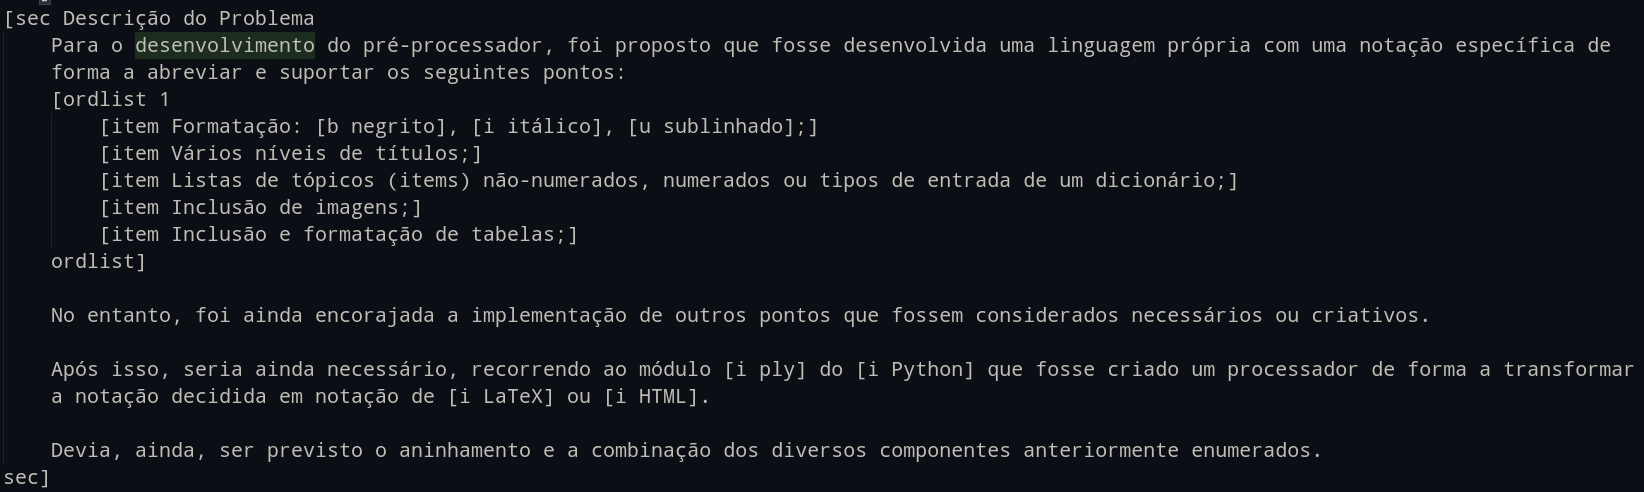
\includegraphics[width=\textwidth]{images/relatorioYA.png}
\caption{Relatório em .YA}
\end{figure}
\\
 
\begin{figure}[!ht]
\centering
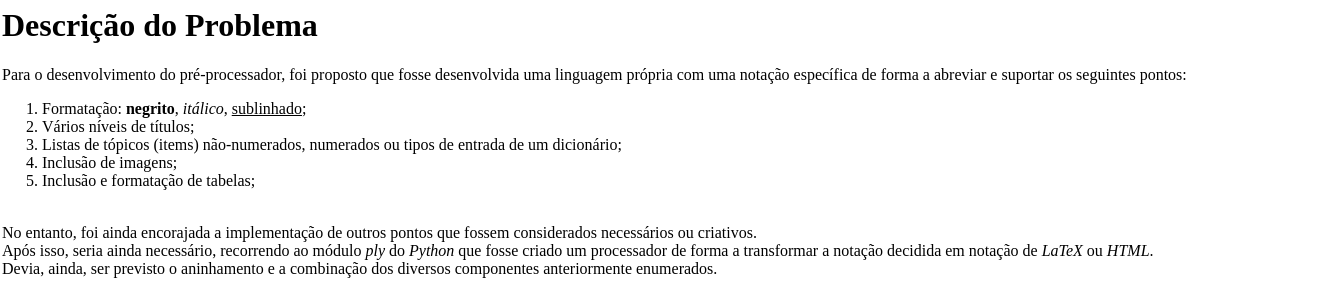
\includegraphics[width=\textwidth]{images/relatorioHTML.png}
\caption{Relatório em HTML}
\end{figure}
\\
 
\begin{figure}[!ht]
\centering
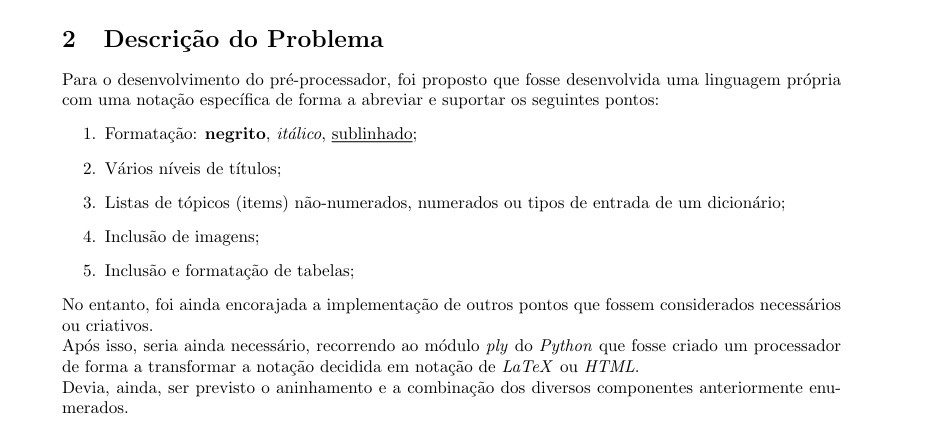
\includegraphics[width=\textwidth]{images/relatorioTEX.png}
\caption{Relatório em Latex}
\end{figure}
 \clearpage
\section{Conclusões e Trabalho Futuro}
Consideramos que o desenvolvimento da aplicação se revela um grande sucesso, tendo o grupo de desenvolvimento sido capaz de implementar as funcionalidades requeridas e outras consideradas interessantes e úteis para uma aplicação deste género.\\
 Assim, podemos concluir que a utilização de Expressões Regulares permite o desenvolvimento de aplicações muito poderosas, sendo, neste caso, suportadas pelos módulos \textit{re} e \textit{ply} do \textit{Python}.\\
 Tal como é normal na indústria do \textit{software}, um programa tem tendência a continuar em desenvolvimento ao longo da sua vida e, assim sendo, consideramos ainda que no futuro esta aplicação poderia ainda almejar à implementação de mais e novas funcionalidades, bem como, do desenvolvimento de \textit{highlighters} de forma a facilitar a escrita dos documentos \textit{.ya}. Para além disso, seria também conveniente implementar \textit{CSS} para tornar os documentos \textit{HTML} mais elegantes.\section{Bibliografia}

\begin{enumerate}
\item \href{https://www.dabeaz.com/ply/ply.html}{Documentação do ply}. Consultado pela última vez a 27 de março de 2022.
\item \href{https://www.w3schools.com/TAgs/default.asp}{W3Schools}. Consultado pela última vez a 27 de março de 2022.
\item \href{https://www.overleaf.com/learn}{Overleaf}. Consultado pela última vez a 27 de março de 2022.
\item \href{https://docs.python.org/3/}{Documentação do Python}. Consultado pela última vez a 27 de março de 2022.
\item José Carlos Ramalho. PPP - Ptext PreProcessor. Consultado pela última vez a 27 de março de 2022.
\end{enumerate}
\end{document}